\section{ESMF Classes}

We divide the ESMF classes into two main categories, those associated with the coupling 
superstructure and those that are part of the utility infrastructure.  Superstructure and data 
classes are based on a hierarchical 
calling tree of increasingly abstract data structures that represent the field data associated 
with the physical systems being modeled.  Utility classes are independent 
of the data classes, though they too have a hierarchical structure; higher-level utilities
employ general-purpose tools such as a message log.

In the listing of classes below we provide a description of each class and its function.

\subsection{Object Model}

The hierarchy of data classes in ESMF is shown in the following UML diagrams.  

\scalebox{0.70}{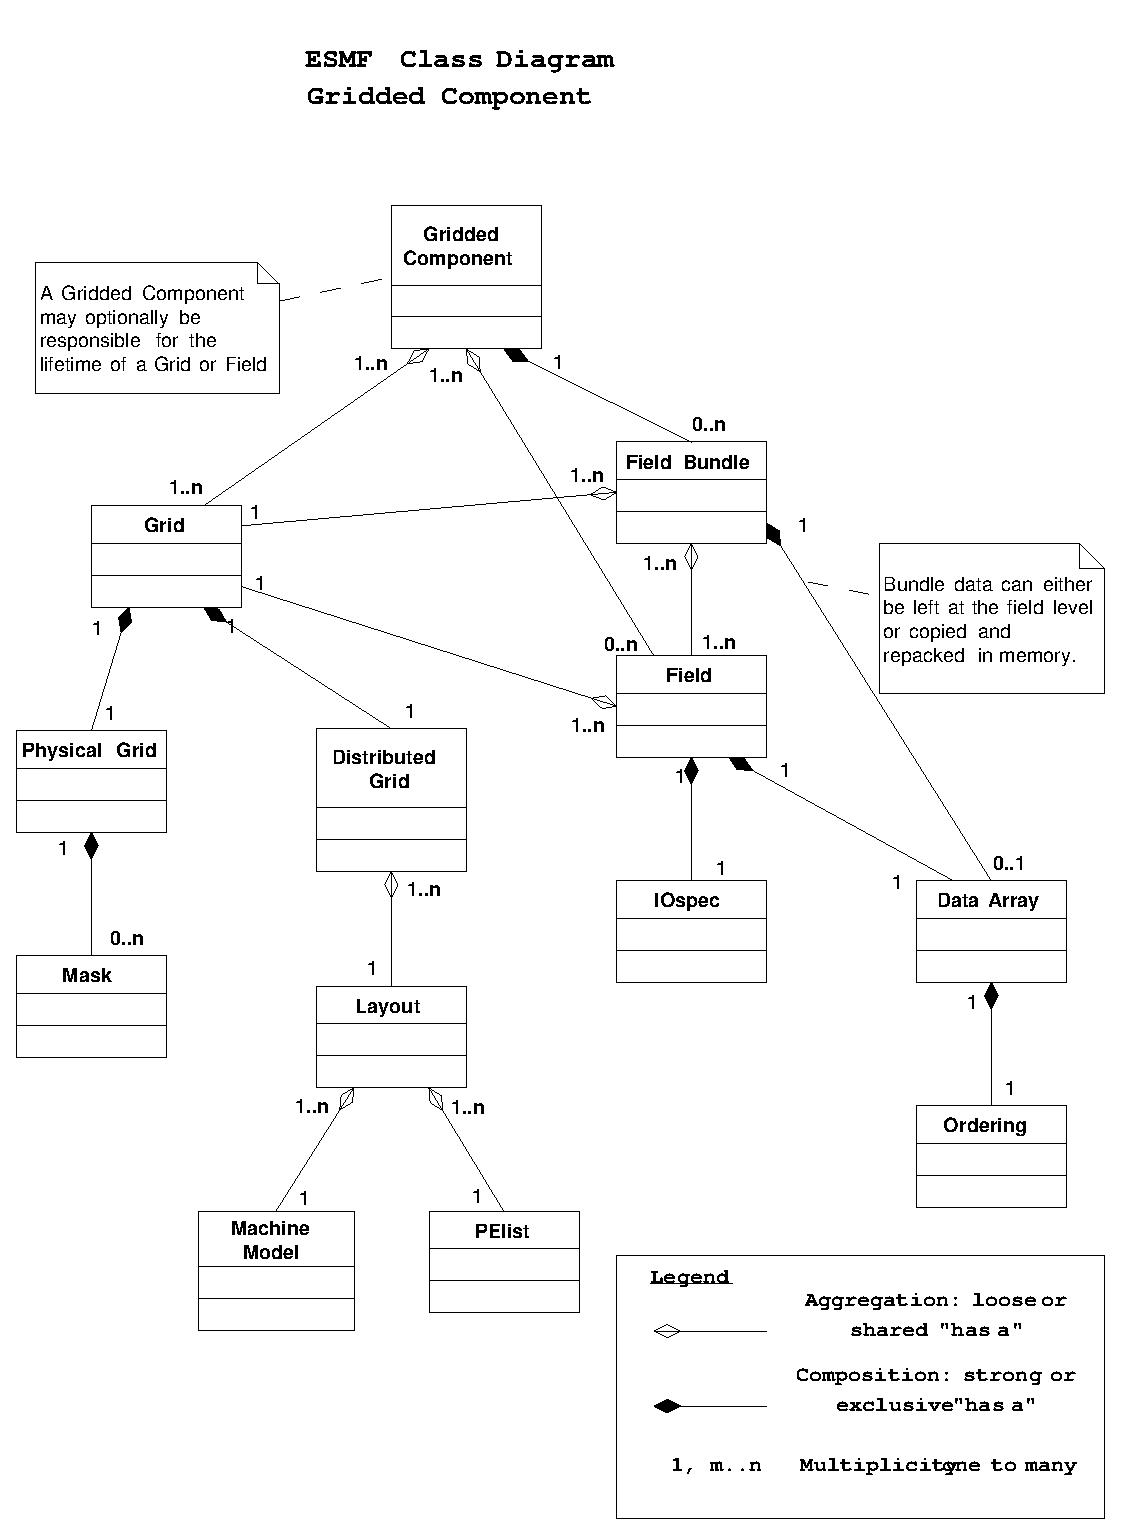
\includegraphics{ESMF_DataStructureHierarchy.eps}}

All objects above are based on the object below.  Attributes
can be handled by generic routines, but it is expected that 
higher level objects will supply their own class specific
methods of the ones listed below.

\scalebox{0.70}{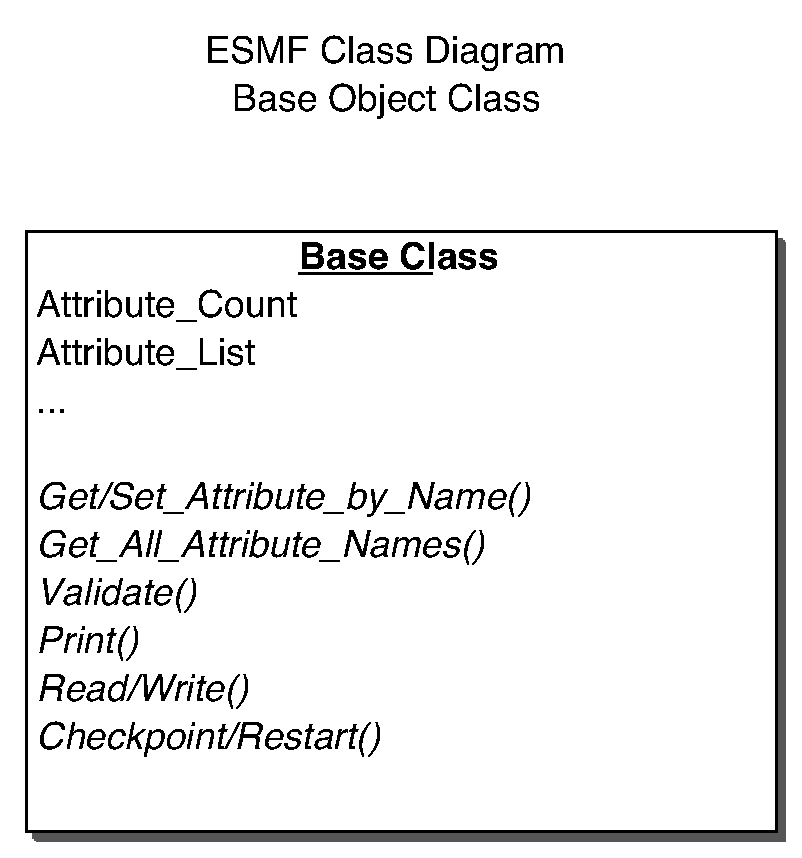
\includegraphics{ESMF_Base.eps}}

Types of components are shown below.

\scalebox{0.70}{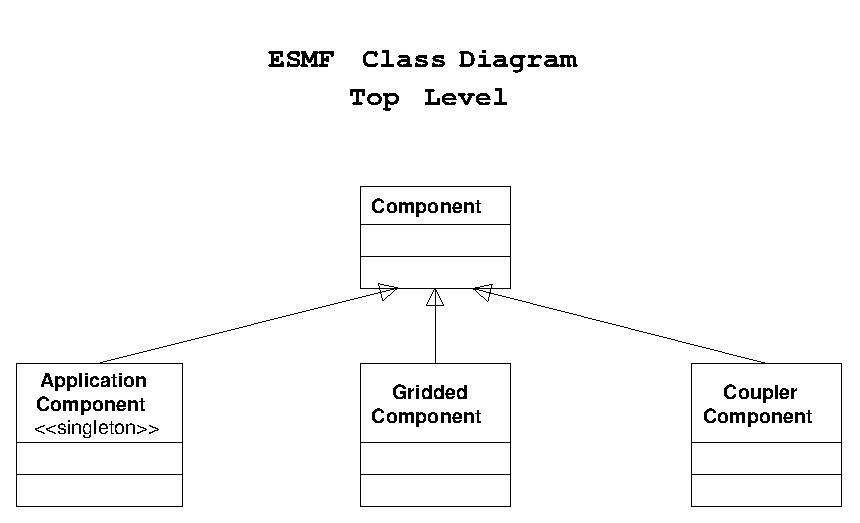
\includegraphics{ESMFTopClassDiagram.eps}}

Coupling diagram.

\scalebox{0.70}{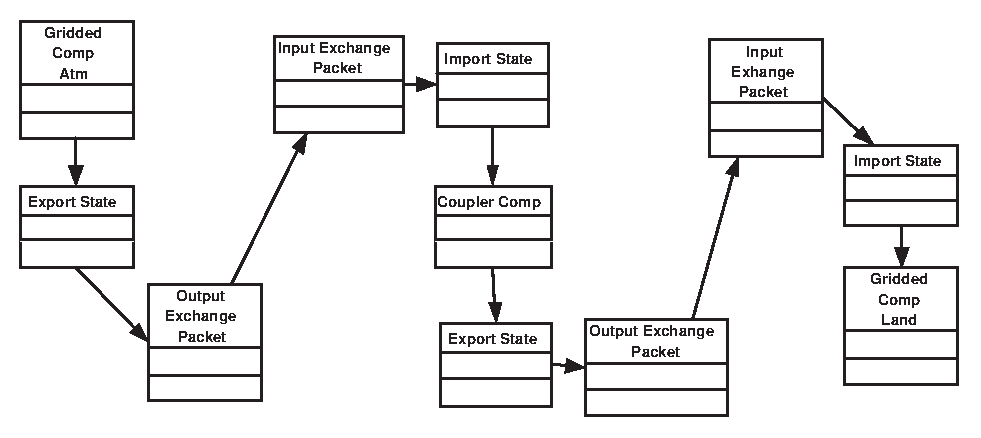
\includegraphics{ESMF_coupler.eps}}

\subsection{Coupling Superstructure}

Below, needs a thorough gutting.

\subsubsection{Component (ESMF\_Comp)} 
\begin{description}
\item [Description] A Component is a functionally related computational entity that represents 
a large system.  
\end{description}

\subsubsection{Application (ESMF\_App)}
\begin{description} 
\item [Description] We define an Application (ESMF\_App) as a special kind of Component 
that is itself composed of a set of sub-Components that interact to form a complete scientific
application.  
\item [Function] The ESMF\_App class is responsible for managing those functions that relate 
to an entire scientific application running under ESMF.  The ESMF\_App initialize method 
must be called at the start of any user application operating under the framework, and
the ESMF\_App finalize method at its end.  At initialization the Application allocates and 
configures any resources needed to run the framework.  The Application also specifies whether 
the system will be brokered using the Registry or not.  The ESMF\_App class can be queried 
for information such as an experiment name, model name, run type (ESMF\_INIT, 
ESMF\_BRANCH, etc.), and for an overall Status.  It can also be queried for
information on any Component that it includes, including its Name, Map, and
Status.
\end{description}

\subsubsection{Coupler Component (ESMF\_Coupler)}
\begin{description}
\item [Description] A Coupler is a specialized type of Component that encompasses all the 
functionality needed to communicate
data between two or more Components. 
\end{description}

\subsubsection{Gridded Component (ESMF\_GComp)} 
\label{sec:gridcomp}
\begin{description}
\item [Description] A Gridded Component is a specialized type of Component that is associated
with a Distributed Grid.  
\end{description}

\subsubsection{Transform (ESMF\_XForm)} 
\begin{description}
\item [Description] A Transform takes one or more physical quantities defined using one set 
of units or representation
and translates them as needed to a different set of units or representation, for example, 
potential temperature
to temperature.  Transform objects are specialized by the application developer.
\item [Function] The Transform class is an abstraction introduced for the
purpose of standardizing high-level coupling interfaces.  It may be overloaded
to take sets of individual Fields or Field Groups.  Methods may include a
separate initialization and run. 
\end{description}

\subsubsection{Layout (ESMF\_Layout)}
\label{sec:layout} 
\begin{description}
\item [Description] A layout is a description of a computational domain that
may describe the decomposition of an Application, a Component, a Field Group, a Field, or 
a Distributed Grid.
If no Layout is specified for an object, it can inherit its layout from an object
higher in the data hierarchy.  
\end{description}

\subsubsection{Distributed Grid (ESMF\_DistGrid)} 

\subsubsection{Field (ESMF\_Field)}
\begin{description} 
\item [Description] A Field represents a single physical field or the components of a 
vector field.  
\end{description}

\subsection{Utility Infrastructure}

\subsubsection{Basic Utilities (ESMF\_BasicUtil)} 
\begin{description}
\item [Description] Utilities that may be utilitized by any other class in the ESMF.  
Collecting these functions into a base-level utility set helps to 
avoid circular referencing.
\item [Function] 
\end{description}

\subsubsection{Basic Communications (ESMF\_BasicComm)}
\begin{description}
\item [Description] This library is a wrapper for MPI and other vendor-supplied 
message passing libraries.
\item [Function] The Basic Communication library provides a generic interface
and efficient communications for the ESMF.  Methods include scatter, gather, send,
receive, synchronize. 
\end{description}

\subsubsection{ (ESMF\_Machine)} 
\begin{description}
\item [Description] The Machine class provides a representation of 
key features of computer hardware and system software.  These
features include memory attributes and configuration, processor type and speed,
interconnect attributes, and system library availability.
\item [Function]
The main purpose of the Machine is to store hardware and system software
information needed by the framework or application programmer in a general
form, but with little abstraction.  This information can be used to perform resource 
allocation, data distribution, and dynamic load balancing.  The Machine can be queried
for platform type(s), number of processors, number of threads, and number of 
nodes.  It may optionally provide information on quantities such as bandwidth and 
latency through active tests.  
\end{description}

\subsubsection{Time Manager (ESMF\_Date, ESMF\_DT)}
\begin{description}
\item [Description] The date and time interval methods in the ESMF provide date
calculations based on a number of different calendars.

\end{description}
















